\documentclass[11pt]{article}

% --- Packages ---
\usepackage[margin=1in]{geometry}
\usepackage[version=4]{mhchem}
\usepackage{chemfig}
\usepackage{amsmath, amssymb}
\usepackage{siunitx}
\usepackage{tcolorbox}
\usepackage{enumitem}
\usepackage{titlesec}
\usepackage{booktabs}
\usepackage{pgfplots}
\pgfplotsset{compat=1.18}

% --- siunitx configuration for Chemistry ---
\DeclareSIUnit\atm{atm}
\DeclareSIUnit\mmHg{mmHg}
\DeclareSIUnit\torr{Torr}

% --- Style Configuration ---
\sisetup{per-mode=symbol}

% Custom tcolorbox styles for distinguishing Provided vs Must Memorize
\tcbset{
    base/.style={fonttitle=\bfseries, left=5pt, right=5pt, top=5pt, bottom=5pt},
    provided/.style={base, colback=blue!5!white, colframe=blue!75!black, title=Key Formula (Provided on Exam)},
    memorize/.style={base, colback=gray!5!white, colframe=gray!50!black, title=Key Formula *}
}

\titleformat{\section}{\large\bfseries\sffamily}{Chapter \thesection:}{1em}{}
\titleformat{\subsection}{\normalsize\bfseries\sffamily}{}{0em}{}

\begin{document}

\title{CHM2045C: Final Exam Comprehensive Study Guide}
\author{Chemistry Study Guide Draft}
\date{Spring 2026}
\maketitle

\section{Foundations: The Chemical Toolbox}

This chapter establishes the fundamental quantitative and qualitative tools required for chemical analysis, focusing on measurement, classification, and naming.

\subsection{Density and Volume Displacement}
Density is an intrinsic property relating mass and volume. For irregular solids, volume is determined by the displacement of a liquid.
\begin{tcolorbox}[memorize]
    \[ d = \frac{m}{V} \quad \text{and} \quad V_{\text{object}} = V_{\text{final}} - V_{\text{initial}} \]
\end{tcolorbox}
\begin{enumerate}
    \item Identify given mass (\si{\gram}) and volume (\si{\milli\liter} or \si{\centi\meter^3}).
    \item Use displacement to find $V$ if necessary (Archimedes' Principle).
    \item Solve for the unknown variable using algebraic rearrangement.
\end{enumerate}

\subsection{Chemical Nomenclature}
\begin{itemize}
    \item \textbf{Ionic Compounds}: Name the cation followed by the anion. Use Roman numerals for transition metals with variable oxidation states (e.g., \ce{FeCl3} is iron(III) chloride).
    \item \textbf{Acids}: Binary acids (\ce{H} + element) use the prefix \textit{hydro-} and suffix \textit{-ic} (e.g., \ce{HCl(aq)} is hydrochloric acid). Oxyacids use \textit{-ic} for \textit{-ate} ions and \textit{-ous} for \textit{-ite} ions.
    \item \textbf{Hydrates}: Append the number of water molecules using Greek prefixes (e.g., \ce{CuSO4.5H2O} is copper(II) sulfate pentahydrate).
\end{itemize}

\subsection{Classification of Matter}
Matter is classified by its composition and uniformity at the particulate level.
\begin{itemize}
    \item \textbf{Elements}: Pure substances consisting of one type of atom (e.g., \ce{O2}).
    \item \textbf{Compounds}: Pure substances with fixed ratios of different atoms (e.g., \ce{H2O}).
    \item \textbf{Mixtures}: Physical blends of substances. \textbf{Homogeneous} (uniform) or \textbf{Heterogeneous} (non-uniform).
\end{itemize}
\begin{center}
    \textit{Particulate Representation of a Water Molecule (\ce{H2O}):} \\
    \vspace{0.5em}
    \chemfig{O(-[1]H)(-[7]H)}
\end{center}

\subsection{Metric System, Units, and Temperature}
Mastery of prefixes is essential for dimensional analysis and unit comparison.
\begin{table}[h]
    \centering
    \begin{tabular}{lcccc}
        \toprule
        Prefix & Nano (n) & Micro ($\mu$) & Milli (m) & Kilo (k) \\
        \midrule
        Factor & $10^{-9}$ & $10^{-6}$ & $10^{-3}$ & $10^{3}$ \\
        \bottomrule
    \end{tabular}
\end{table}

\begin{tcolorbox}[provided, title=Temperature Conversion (Provided)]
    \[ T_{\si{\kelvin}} = T_{^\circ\text{C}} + 273.15 \]
\end{tcolorbox}
\textbf{Note}: Kelvin is mandatory for all gas law and thermodynamic calculations. Absolute zero is \SI{0}{\kelvin}.

\newpage

\section{Atomic Structure}

Understanding the atom involves identifying its constituent subatomic particles and their contribution to the element's identity and mass.

\subsection{Nuclide Notation and Subatomic Particles}
The identity of an atom is defined by its atomic number ($Z$), while its mass is determined by the sum of protons and neutrons.
\begin{tcolorbox}[memorize]
    \[ A = Z + N \quad \text{and} \quad \text{Charge} = \text{Protons} - \text{Electrons} \]
\end{tcolorbox}
In the symbol \ce{^{A}_{Z}X^{charge}}:
\begin{itemize}
    \item \textbf{Protons}: Equal to $Z$ (Atomic Number). Defines the element.
    \item \textbf{Neutrons}: Calculated as $A - Z$ (Mass Number - Atomic Number).
    \item \textbf{Electrons}: Calculated as $Z - (\text{Charge})$. In neutral atoms, $e^- = p^+$.
\end{itemize}

\subsection{Average Atomic Mass}
The mass reported on the periodic table is a weighted average of all naturally occurring isotopes based on their abundance.
\begin{tcolorbox}[memorize]
    \[ \text{Avg. Atomic Mass} = \sum_{i} (\text{Mass of Isotope}_i \times \text{Fractional Abundance}_i) \]
\end{tcolorbox}
\textbf{Technique}: Convert percentages to decimals (e.g., $75\% \rightarrow 0.75$) to find the "fractional abundance" before multiplying by isotopic mass.

\subsection{Isotopes vs. Ions}
\begin{itemize}
    \item \textbf{Isotopes}: Atoms of the same element (same $Z$) with different numbers of neutrons ($N$), resulting in different mass numbers ($A$).
    \item \textbf{Ions}: Atoms that have gained or lost electrons, resulting in a net positive (cation) or negative (anion) charge.
\end{itemize}

\newpage

\section{Electronic Structure and Periodic Trends}

\subsection{Electromagnetic Radiation and the Bohr Model}
Light behaves as both a wave and a particle (photon). The energy of an electron in an atom is quantized.
\begin{tcolorbox}[memorize, title=Light and Photon Energy *]
    \[ c = \lambda \nu \quad \text{and} \quad E = h\nu = \frac{hc}{\lambda} \]
    \[ \Delta E = -2.18 \times 10^{-18} \si{\joule} \left( \frac{1}{n_f^2} - \frac{1}{n_i^2} \right) \]
\end{tcolorbox}
Note: $h$ and $c$ are usually provided, but the relationships between $E$, $\lambda$, and $\nu$ must be mastered.

\subsection{Quantum Numbers}
Four quantum numbers describe the unique quantum state (or "address") of an electron:
\begin{enumerate}
    \item \textbf{Principal ($n$)}: Energy level ($1, 2, 3 \dots$).
    \item \textbf{Angular Momentum ($l$)}: Orbital shape ($0$ to $n-1$). $s=0, p=1, d=2, f=3$.
    \item \textbf{Magnetic ($m_l$)}: Orbital orientation ($-l$ to $+l$).
    \item \textbf{Spin ($m_s$)}: Direction of electron spin ($+1/2$ or $-1/2$).
\end{enumerate}

\subsection{Electron Configurations}
Follow three core principles to populate orbitals in the ground state:
\begin{itemize}
    \item \textbf{Aufbau Principle}: Electrons fill the lowest energy orbitals first ($1s, 2s, 2p \dots$).
    \item \textbf{Pauli Exclusion Principle}: No two electrons can have the same four quantum numbers (max 2 $e^-$ per orbital with opposite spins).
    \item \textbf{Hund's Rule}: Electrons fill degenerate orbitals singly with parallel spins before pairing.
\end{itemize}
\textbf{Noble Gas Shorthand}: Use the preceding noble gas to represent core electrons (e.g., \ce{Sn} is \ce{[Kr] 5s^2 4d^{10} 5p^2}).

\subsection{Periodic Trends: Ionization Energy (IE)}
Ionization Energy is the energy required to remove an electron from a gaseous atom.
\begin{itemize}
    \item \textbf{Across a Period}: IE generally increases due to increasing effective nuclear charge ($Z_{\text{eff}}$).
    \item \textbf{Down a Group}: IE generally decreases due to increasing atomic radius and electronic shielding.
\end{itemize}

\newpage

\section{Formula Calculations and the Mole}

\subsection{Core Concepts}
The mole is the fundamental unit in chemistry for measuring the amount of a substance. It provides a bridge between the microscopic world of atoms and molecules and the macroscopic world of grams and liters.

\begin{itemize}[noitemsep]
    \item \textbf{Avogadro's Number}: $1 \text{ mole} = \num{6.022e23}$ representative particles.
    \item \textbf{Molar Mass}: The mass in grams of one mole of a substance (\si{\gram\per\mole}).
    \item \textbf{Percent Composition}: The percentage by mass of each element in a compound.
\end{itemize}

\begin{tcolorbox}[provided, title=Avogadro Constant (Provided)]
    \[ N_A = \num{6.022e23} \si{\per\mole} \]
\end{tcolorbox}

\begin{tcolorbox}[memorize, title=Mole Calculations *]
    \[ n = \frac{m}{MM} \quad \text{and} \quad N = n \times N_A \]
\end{tcolorbox}

\subsection{Problem-Solving Skills}
\begin{enumerate}
    \item \textbf{Mass-to-Particle Conversions}:
    \begin{itemize}
        \item $\text{Mass (g)} \xrightarrow{\div MM} \text{Moles} \xrightarrow{\times N_A} \text{Particles}$
    \end{itemize}
    
    \item \textbf{Calculating Empirical Formulas}:
    \begin{enumerate}[label=\alph*)]
        \item Assume a \SI{100}{\gram} sample (convert \% directly to grams).
        \item Convert grams of each element to moles using atomic masses.
        \item Divide all mole values by the smallest mole value obtained.
        \item If necessary, multiply by a small integer to reach whole numbers.
    \end{enumerate}

    \item \textbf{Percent Mass Composition}:
    \begin{tcolorbox}[memorize]
        \[ \text{Mass \% of element} = \left( \frac{\text{mass of element in 1 mol compound}}{\text{molar mass of compound}} \right) \times 100\% \]
    \end{tcolorbox}
\end{enumerate}

\newpage

\section{Stoichiometry}

\subsection{Core Concepts}
Stoichiometry involves using the relationships between reactants and products in a balanced chemical equation to determine quantitative data.

\begin{itemize}
    \item \textbf{Mole Ratio}: Derived from the coefficients of a balanced equation; it is the "bridge" that allows conversion between different substances.
    \item \textbf{Limiting Reactant}: The reactant that is completely consumed first, limiting the amount of product formed.
    \item \textbf{Theoretical Yield}: The maximum amount of product that can be produced from a given amount of limiting reactant.
\end{itemize}

\begin{tcolorbox}[memorize, title=Reaction Efficiency *]
    \[ \text{Percent Yield} = \left( \frac{\text{Actual Yield}}{\text{Theoretical Yield}} \right) \times 100\% \]
\end{tcolorbox}

\subsection{Problem-Solving Skills}
\begin{enumerate}
    \item \textbf{Mass-to-Mass Stoichiometry}:
    \begin{itemize}
        \item $\text{Mass A} \xrightarrow{\div MM_A} \text{Moles A} \xrightarrow{\text{Mole Ratio}} \text{Moles B} \xrightarrow{\times MM_B} \text{Mass B}$
    \end{itemize}

    \item \textbf{Identifying the Limiting Reactant}:
    \begin{enumerate}[label=\alph*)]
        \item Convert the given amounts of all reactants to moles.
        \item Divide the moles of each reactant by its coefficient in the balanced equation.
        \item The reactant with the smallest resulting value is the \textbf{limiting reactant}.
    \end{enumerate}

    \item \textbf{Calculating Theoretical Yield}:
    \begin{itemize}
        \item Use the moles of the limiting reactant and the mole ratio from the balanced equation to find the moles (and then mass) of the desired product.
    \end{itemize}
\end{enumerate}

\newpage

\section{Solutions and Aqueous Reactions}

\subsection{Core Concepts}
Most chemical reactions occur in solution. Understanding concentration and the behavior of ions in water is critical.

\begin{itemize}
    \item \textbf{Molarity (M)}: A measure of concentration defined as moles of solute per liter of solution (\si{\mole\per\liter}).
    \item \textbf{Electrolytes}: Substances that dissociate into ions in water (Strong = complete dissociation, Weak = partial).
    \item \textbf{Precipitation}: A reaction where two aqueous solutions form an insoluble solid product.
    \item \textbf{Oxidation States}: Bookkeeping for electrons to track redox processes.
\end{itemize}

\begin{tcolorbox}[memorize, title=Concentration and Dilution *]
    \[ M = \frac{n}{V} \quad \text{and} \quad M_1V_1 = M_2V_2 \]
\end{tcolorbox}

\subsection{Solubility Reference}
\begin{table}[h]
    \centering
    \caption{Solubility Guidelines for Ionic Compounds *}
    \begin{tabular}{ll}
        \toprule
        \textbf{Always Soluble} & \ce{NO3-}, \ce{C2H3O2-}, Group 1 (\ce{Li+}, \ce{Na+}, \ce{K+}), \ce{NH4+} \\
        \midrule
        \textbf{Generally Soluble} & \ce{Cl-}, \ce{Br-}, \ce{I-} (except \ce{Ag+}, \ce{Pb^{2+}}, \ce{Hg2^{2+}}) \\
                                  & \ce{SO4^{2-}} (except \ce{Ba^{2+}}, \ce{Sr^{2+}}, \ce{Ca^{2+}}, \ce{Pb^{2+}}, \ce{Ag+}) \\
        \midrule
        \textbf{Generally Insoluble} & \ce{S^{2-}}, \ce{OH-} (except Group 1, \ce{NH4+}; \ce{Ca^{2+}}, \ce{Sr^{2+}}, \ce{Ba^{2+}} are soluble) \\
                                    & \ce{CO3^{2-}}, \ce{PO4^{3-}} (except Group 1 and \ce{NH4+}) \\
        \bottomrule
    \end{tabular}
\end{table}

\subsection{Problem-Solving Skills}
\begin{enumerate}
    \item \textbf{Writing Net Ionic Equations}:
    \begin{enumerate}[label=\alph*)]
        \item Write the balanced molecular equation.
        \item Use solubility rules to identify precipitates (\ce{(s)}) and aqueous species (\ce{(aq)}).
        \item Write the complete ionic equation (dissociate all strong electrolytes).
        \item Cancel \textbf{spectator ions} (ions that appear identical on both sides).
    \end{enumerate}

    \item \textbf{Assigning Oxidation States}:
    \begin{itemize}
        \item Elements in standard state = 0; Monoatomic ions = charge.
        \item \ce{F} = -1; \ce{O} = -2 (usually); \ce{H} = +1 (with non-metals).
        \item The sum of oxidation states must equal the overall charge of the molecule/ion.
    \end{itemize}

    \item \textbf{Solution Stoichiometry \& Titration}:
    \begin{itemize}
        \item Use volume and molarity to find moles ($n = M \times V$).
        \item Apply stoichiometry from the balanced neutralization equation (e.g., \ce{HCl + NaOH -> NaCl + H2O}).
        \item At the equivalence point: $\text{moles H}^+ = \text{moles OH}^-$.
    \end{itemize}
\end{enumerate}

\newpage

\section{Heat and Enthalpy}

\subsection{Core Concepts}
\begin{itemize}
    \item \textbf{Calorimetry}: The measurement of heat flow into or out of a system during a chemical or physical process.
    \item \textbf{Conservation of Energy}: In an insulated system, heat lost by one component is gained by another: $-q_{\text{lost}} = q_{\text{gained}}$.
    \item \textbf{Standard Enthalpy of Formation ($\Delta H_f^\circ$)}: The change in enthalpy when 1 mole of a substance is formed from its elements in their standard states. Note: $\Delta H_f^\circ = 0$ for any element in its most stable form (e.g., \ce{O2(g)}, \ce{C(graphite)}).
    \item \textbf{Hess's Law}: If a reaction is carried out in a series of steps, $\Delta H$ for the overall reaction equals the sum of the enthalpy changes for the individual steps.
\end{itemize}

\subsection{Calorimetry}
\begin{tcolorbox}[provided, title=Specific Heat Equation (Provided)]
    \[ q = m c_s \Delta T \]
\end{tcolorbox}

\subsection{Reaction Enthalpy Calculations}
\begin{tcolorbox}[memorize, title=Enthalpy Calculations *]
    \textbf{From Heats of Formation}:
    \[ \Delta H_{\text{rxn}}^\circ = \sum n\Delta H_f^\circ(\text{products}) - \sum m\Delta H_f^\circ(\text{reactants}) \]
    \vspace{0.2em}
    \textbf{From Bond Energies}:
    \[ \Delta H_{\text{rxn}}^\circ = \sum (\text{bonds broken}) - \sum (\text{bonds formed}) \]
\end{tcolorbox}
\textbf{Crucial Distinction}: Formation uses (Products - Reactants), while Bond Energy uses (Reactants/Broken - Products/Formed).

\subsection{Problem-Solving Skills}
\begin{enumerate}
    \item \textbf{Calculating Reaction Enthalpy}:
        \begin{itemize}
            \item Identify $\Delta H_f^\circ$ for all species. Pure elements in standard states are \SI{0}{\kilo\joule\per\mole}.
            \item Multiply each value by its stoichiometric coefficient.
            \item Apply: $\text{Products} - \text{Reactants}$.
        \end{itemize}
    \item \textbf{Applying Hess's Law}:
        \begin{itemize}
            \item If you reverse a reaction, flip the sign of $\Delta H$.
            \item If you multiply coefficients by a factor $n$, multiply $\Delta H$ by $n$.
            \item Sum the modified $\Delta H$ values to find the target enthalpy.
        \end{itemize}
\end{enumerate}

\newpage

\section{Structure and Bonding}

\subsection{Core Concepts}
\begin{itemize}
    \item \textbf{Formal Charge}: Used to determine the most plausible Lewis structure. The best structure minimizes formal charges and places negative charges on the most electronegative atoms.
    \item \textbf{Lattice Energy}: The energy required to separate 1 mole of an ionic solid into gaseous ions. It increases with increasing ion charge and decreasing ion size.
    \item \textbf{VSEPR Theory}: Predicts molecular shape based on the repulsion between electron domains (bonding pairs and lone pairs).
    \item \textbf{Hybridization}: The mixing of atomic orbitals to form new hybrid orbitals (e.g., $sp, sp^2, sp^3$) suitable for bonding.
\end{itemize}

\subsection{Lattice Energy and Formal Charge}
\begin{tcolorbox}[memorize, title=Coulomb's Law *]
    \[ E_{\text{lattice}} \propto \frac{Q_1 Q_2}{d} \]
\end{tcolorbox}

\begin{tcolorbox}[memorize, title=Formal Charge *]
    \[ FC = (\text{Valence } e^-) - (\text{Non-bonding } e^-) - \frac{1}{2}(\text{Bonding } e^-) \]
\end{tcolorbox}

\subsection{Molecular Geometry Example: Tetrahedral}
Centrally bonded atoms with four electron domains (e.g., \ce{CH4}) adopt a tetrahedral geometry with bond angles of approximately \SI{109.5}{\degree}.

\begin{center}
    \chemfig{C(-[2]H)(<:[5]H)(<[6]H)(-[0]H)}
    \quad
    \textit{Tetrahedral Geometry (\ce{CH4})}
\end{center}

\subsection{Problem-Solving Skills}
\begin{enumerate}
    \item \textbf{Determining Hybridization}: Count electron domains (lone pairs + bonding regions).
        \begin{itemize}
            \item 2 domains: $sp$ (Linear)
            \item 3 domains: $sp^2$ (Trigonal Planar)
            \item 4 domains: $sp^3$ (Tetrahedral)
        \end{itemize}
    \item \textbf{Bond Counting}: Every single bond is 1 $\sigma$. Double bonds consist of 1 $\sigma$ and 1 $\pi$. Triple bonds consist of 1 $\sigma$ and 2 $\pi$.
\end{enumerate}

\newpage

\section{States of Matter}

\subsection{Core Concepts}
\begin{itemize}
    \item \textbf{Ideal Gas Law}: Relates pressure, volume, temperature, and moles. Assumes gas particles have no volume and no IMFs.
    \item \textbf{Kinetic Molecular Theory (KMT)}: Gas particles are in constant random motion. Temperature is a measure of average kinetic energy.
    \item \textbf{Intermolecular Forces (IMFs)}:
        \begin{itemize}
            \item \textbf{London Dispersion}: Present in all molecules; strength increases with polarizability (larger electron clouds).
            \item \textbf{Dipole-Dipole}: Between polar molecules.
            \item \textbf{Hydrogen Bonding}: Strong dipole-dipole interaction involving H bonded to N, O, or F.
        \end{itemize}
\end{itemize}

\subsection{Gas Laws and Constants}
\begin{tcolorbox}[provided, title=Gas Laws and Constants (Provided)]
    \textbf{Constants}:
    \[ R = \SI{0.0821}{\liter\atm\per\mole\per\kelvin} \]
    \[ 1 \text{ atm} = 760 \text{ mmHg} = 760 \text{ Torr} \]
    \vspace{0.5em}
    \textbf{Laws}:
    \[ PV = nRT \quad \text{and} \quad \frac{P_1V_1}{n_1T_1} = \frac{P_2V_2}{n_2T_2} \]
    \vspace{0.5em}
    \textbf{Graham's Law of Effusion}:
    \[ \frac{\text{rate}_1}{\text{rate}_2} = \sqrt{\frac{M_2}{M_1}} \]
\end{tcolorbox}

\subsection{Gas Density}
\begin{tcolorbox}[memorize, title=Gas Density *]
    \[ d = \frac{PM}{RT} \]
\end{tcolorbox}

\subsection{Maxwell-Boltzmann Distribution}
The distribution of molecular speeds changes with temperature. At higher temperatures, the peak shifts right (higher average speed) and flattens (wider distribution of speeds).

\begin{center}
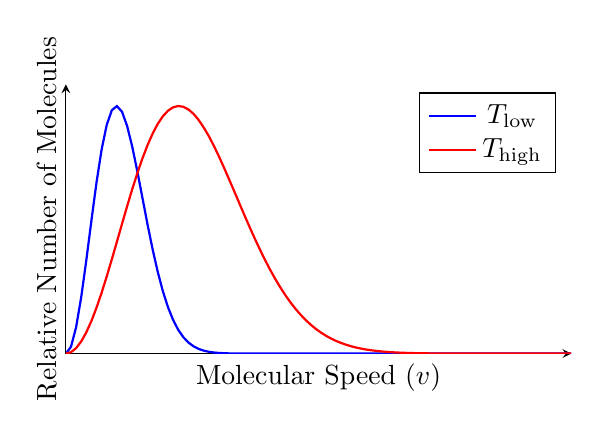
\begin{tikzpicture}
\begin{axis}[
    axis lines = left,
    xlabel = {Molecular Speed ($v$)},
    ylabel = {Relative Number of Molecules},
    ticks = none,
    xmin = 0, xmax = 10,
    ymin = 0, ymax = 1.6,
    width = 8cm, height = 5cm,
    legend pos = north east
]
% Low Temperature (T1)
\addplot [domain=0:10, samples=100, thick, blue] {4*x^2*exp(-x^2)};
\addlegendentry{$T_{\text{low}}$}
% High Temperature (T2)
\addplot [domain=0:10, samples=100, thick, red] {0.8*x^2*exp(-0.2*x^2)};
\addlegendentry{$T_{\text{high}}$}
\end{axis}
\end{tikzpicture}
\end{center}

\subsection{Problem-Solving Skills}
\begin{enumerate}
    \item \textbf{Gas Law Calculations}: Always convert temperature to \si{\kelvin} ($T_K = T_C + 273.15$). Ensure units match the $R$ constant.
    \item \textbf{Predicting Physical Properties}: Stronger IMFs result in higher boiling points, higher melting points, and lower vapor pressures.
\end{enumerate}

\newpage

\section*{Addendum: Exam Formula \& Constant Reference}

\subsection*{Provided Information}
\begin{itemize}
    \item \textbf{Temperature}: $T_{\si{\kelvin}} = T_{^\circ\text{C}} + 273.15$
    \item \textbf{Avogadro Constant}: $N_A = \num{6.022e23} \si{\per\mole}$
    \item \textbf{Gas Constant}: $R = \SI{0.0821}{\liter\atm\per\mole\per\kelvin}$
    \item \textbf{Pressure}: $\SI{1}{\atm} = \SI{760}{\mmHg} = \SI{760}{\torr}$
    \item \textbf{Ideal Gas Law}: $PV = nRT$
    \item \textbf{Combined Gas Law}: $\frac{P_1V_1}{n_1T_1} = \frac{P_2V_2}{n_2T_2}$
    \item \textbf{Graham's Law}: $\frac{\text{rate}_1}{\text{rate}_2} = \sqrt{\frac{M_2}{M_1}}$
    \item \textbf{Specific Heat}: $q = m c_s \Delta T$
\end{itemize}

\subsection*{Information to Memorize *}
\begin{itemize}
    \item \textbf{Atomic Mass}: $\sum (\text{mass} \times \text{fraction abundance})$
    \item \textbf{Light}: $c = \lambda \nu$ and $E = h\nu = hc/\lambda$
    \item \textbf{Rydberg}: $\Delta E = -2.18 \times 10^{-18} \si{\joule} (1/n_f^2 - 1/n_i^2)$
    \item \textbf{Molarity}: $M = n/V$
    \item \textbf{Enthalpy (Formation)}: $\sum \Delta H_f^\circ(\text{prod}) - \sum \Delta H_f^\circ(\text{react})$
    \item \textbf{Enthalpy (Bonds)}: $\sum (\text{broken}) - \sum (\text{formed})$
    \item \textbf{Lattice Energy}: $E \propto Q_1Q_2/d$
    \item \textbf{Solubility}: (See Table in Chapter 6)
\end{itemize}

\end{document}
